%%%%%%%%%%%% Attribution %%%%%%%%%%%%
% This template was created by 
% Chuck F. Rocca at WCSU and may be
% copied and used freely for 
% non-commercial purposes.
% 10-17-2021
%%%%%%%%%%%%%%%%%%%%%%%%%%%%%%%%%%%%%

%%%%%%% Start Document Header %%%%%%%
% In creating a new document
% copy and paste the header 
% as is.
%%%%%%%%%%%%%%%%%%%%%%%%%%%%%%%%%%%%%

\documentclass[12pt]{article}

%%%% Header Information %%%%
    %%% Document Settings %%%%
    \usepackage[utf8]{inputenc}
    \usepackage[
        twoside,
        top=1in,
        bottom=0.75in,
        inner=0.5in,
        outer=0.5in
    ]{geometry}
    \pagestyle{myheadings}

%%%% Additional Commands to Load %%%%
    \usepackage{tcolorbox}
    \tcbuselibrary{skins}
    \usepackage{minted}
    \usepackage{color}
    \usepackage{tikz}
    \usetikzlibrary{calc}
    \usepackage{tabularx,colortbl}
    \usepackage{amsfonts,amsmath,amssymb}
    \usepackage{titling}
    \usepackage{mathrsfs}
    \usepackage{calc}
    \usepackage{xepersian}

%%%% Commands to Define Homework Boxes %%%%
%%%% Box Definition %%%%
    \newtcolorbox{prob}[1]{
    % Set box style
        sidebyside,
        sidebyside align=bottom,
    % Dimensions and layout
        width=\textwidth,
        toptitle=2.5pt,
        bottomtitle=2.5pt,
        righthand width=0\textwidth,
    % Coloring
        colbacktitle=gray!30,
        coltitle=black,
        colback=white,
        colframe=white,
    % Title formatting
        title={
            #1 \hfill نمره:\phantom{WWWW}
        },
        fonttitle=\large\bfseries
    }

%%%% Environment Definition %%%%
    \newenvironment{problem}[1]{
        \begin{prob}{#1}
    }
    {
        \tcblower
        \centering
        \vspace{\baselineskip}
        \end{prob}
    }



%%%% Document Information %%%%
    \title{\lr{HW4 Solutions}}
    \date{}
    \author{\lr{Written By Reza Shahriari}}

%%%%%%% End Document Header %%%%%%%


%%%% Begin Document %%%%
% note that the document starts with
% \begin{document} and ends with
% \end{document}
%%%%%%%%%%%%%%%%%%%%%%%%
\settextfont{BNAZANIN.TTF}

\begin{document}

%%%% Format Running Header %%%%%
\markboth{\theauthor}{\thetitle}

%%%% Insert the Title Information %%%
\maketitle


%%%% General Description of the Document %%%%
\centering
\lr{Disclaimer:} 

\lr{This is the solution manual to the homework assigned to students of Digital Control - Dr.Talebi.}

\lr{We do not guarantee that this solution is precise and thorough so please contact your TA to propose your innovative solutions and/or any probable mistakes.}


%%%% Introduction to the General Template %%%%

 \begin{problem}{سوال اول}
 	    	\raggedleft
 	\lr{We have the following:}
 	
 	\lr{We have used a better approach in analyzing the stability of the equation in this question.}
 	
 	$a_0 = 0.3 , a_1 = -0.1 , a_2 = -1.1 , a_3 = 1$
 	
 	\lr{First check the stability criterion below:}
 	
 	\centering
 	$1. D(1) > 0$
 	
 	$2. (-1)^nD(-1) > 0$
 	
 	$3. |a_3| > |a_0|$
 	
 	$4. |b_0| > |b_2| $
 	
 	\raggedleft
 	
 	$1. D(1) = 1 - 1.1 - 0.1 + 0.3 = 0.1 > 0$
 	
 	$2. (-1)^3 D(-1) = (-1)(-1 -1.1 +0.1 +0.3) > 0$
 	
 	$3.\left| {{a}_{3}} \right|>\left| {{a}_{0}} \right|\to 1>0.3$
 	
 	\raggedleft
 	\lr{Construct the Jury's array:}
 	
 	\centering
 	\[\begin{matrix}
 		{{z}^{0}} & {{z}^{1}} & {{z}^{2}} & {{z}^{3}}  \\
 		0.3 & -0.1 & -1.1 & 1  \\
 		1 & -1.1 & -0.1 & 0.3  \\
 		\begin{matrix}
 			{{b}_{0}}  \\
 			{}  \\
 		\end{matrix} & \begin{matrix}
 			{{b}_{1}}  \\
 			{}  \\
 		\end{matrix} & \begin{matrix}
 			{{b}_{2}}  \\
 			{}  \\
 		\end{matrix} & {}  \\
 	\end{matrix}\]
 	
 	\raggedleft
 	
 	${{b}_{0}}=\left| \begin{matrix}
 		0.3 & 1  \\
 		1 & 0.3  \\
 	\end{matrix} \right| = 0.91$
 	
 	${{b}_{2}}=\left| \begin{matrix}
 		0.3 & -0.1  \\
 		1 & -1.1  \\
 	\end{matrix} \right| = -0.23$
 	
 	$|b_0| > |b_2|$
 	
 	\lr{Thus the system is stable.}
 	
    \end{problem}
    
    \begin{problem}{سوال دوم}
    	\raggedleft
    	\lr{We have the following:}
    	
    	$a_0 = -0.35 , a_1 = 1.55 , a_2 = -2.2 , a_3 = 1$
    	
    	\lr{First check the stability criterion below:}
    	
    	\centering
    	$1. D(1) > 0$
    	
    	$2. (-1)^nD(-1) > 0$
    	
    	$3. |a_3| > |a_0|$
    	
    	$4. |b_0| > |b_2| $
    	
    	\raggedleft
    	$1. D(1) = 1-2.2+1.55-0.35 = 0$
    	
    	\lr{The condition is not strictly satisfied, and for a definitive answer it must be checked.}
    	
    	
    	$2. (-1)^nD(-1) =  (-1)^3(-1-2.2-1.55-0.35) > 0$
    	
    	$3. |a_3| > |a_0| , 1 > 0.35$
    	
    	$4. |b_0| > |b_2| $
    	
    	\lr{Construct the Jury array:}
    	
    	\centering
    	\[\begin{matrix}
    		{{z}^{0}} & {{z}^{1}} & {{z}^{2}} & {{z}^{3}}  \\
    		-0.35 & 1.55 & -2.2 & 1  \\
    		1 & -2.2 & 1.55 & -0.35  \\
    		\begin{matrix}
    			{{b}_{0}}  \\
    			{}  \\
    		\end{matrix} & \begin{matrix}
    			{{b}_{1}}  \\
    			{}  \\
    		\end{matrix} & \begin{matrix}
    			{{b}_{2}}  \\
    			{}  \\
    		\end{matrix} & {}  \\
    	\end{matrix}\]
    	
    	\raggedleft
    	${{b}_{0}}=\left| \begin{matrix}
    		-0.35 & 1  \\
    		1 & -0.35  \\
    	\end{matrix} \right| = -0.8775$
    	
    	${{b}_{2}}=\left| \begin{matrix}
    		-0.35 & 1.55  \\
    		1 & -2.2  \\
    	\end{matrix} \right| = -0.78$
    	
    	$|b_0| > |b_2|$
    
    	\lr{The final analysis of stability requires a resize of the unit circle.}

    	\lr{First let's make the unit circle bigger:}
    	
    	$z^n \to (1+n\epsilon)z^n$
    	
    	$D(z)_{new} = (1+3\epsilon)z^3 + -2.2(1+2\epsilon)z^2 + 1.55(1+\epsilon)z -0.35  $
    	
    	\lr{Evaluate the Jury's necessary conditions:}
    	
    	$D(1)_{new} = 1 + 3\epsilon - 2.2 -4.4\epsilon + 1.55 + 1.55\epsilon - 0.35$
    	
    	$D(1)_{new} = 0.15\epsilon$
    	
    	\lr{since $\epsilon$ is positive $D(1)_{new}$ is positive. So the necessary conditions of Jury is satisfied for the "slightly bigger unit circle"}
    	
    	\lr{Now let us do the same thing with the "slightly smaller unit circle"}
    	
    	$z^n \to (1-n\epsilon)z^n$
    	
    	$D(z)_{new} = (1-3\epsilon)z^3 + -2.2(1-2\epsilon)z^2 + 1.55(1-\epsilon)z -0.35  $
    	
    	$D(1)_{new} = 1 - 3\epsilon - 2.2 +4.4\epsilon + 1.55 - 1.55\epsilon - 0.35$
    	
    	$D(1)_{new} = -0.15\epsilon$
    	
    	\lr{since $\epsilon$ is positive $D(1)_{new}$ is negative. So the necessary conditions of Jury is not satisfied for the "slightly smaller unit circle", hence we have a pole on the unit circle.}
    	
    \end{problem}
    
    \begin{problem}{سوال سوم}
    	\raggedleft
    	\lr{First obtain the discrete transfer function for the given sampling period.}
    	
    	\begin{align}
    		& G(z)=Z\left\{ \frac{1-{{e}^{-Ts}}}{s}\times \frac{K}{s(s+1)} \right\} \nonumber \\ 
    		& G(z)=(1-{{z}^{-1}})\left\{ \frac{K}{{{s}^{2}}(s+1)} \right\}\xrightarrow{T=2} \nonumber \\ 
    		& G(z)=\frac{1.1353K(z+0.5232)}{(z-1)(z-0.1353)} \nonumber \\ 
    		& \nonumber
    	\end{align}
    	
    	\lr{Which has one zero at z = 0.5232 and two poles at z = 1 and z = 0.1353}
    	
    	\lr{The two breaking points are 0.4783 and -1.52}
    	
    	\lr{the root locus can be as below:}
    	
    	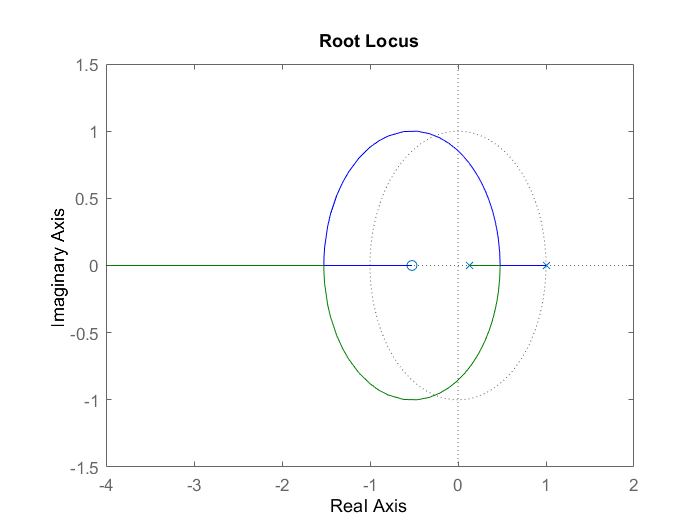
\includegraphics[width= \linewidth]{Resources/3.png}
    	
    \end{problem}
    \begin{figure}
    	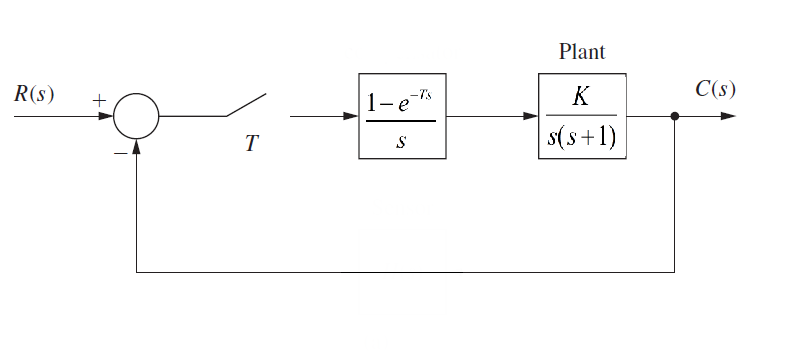
\includegraphics[width=\linewidth]{Resources/1.png}
    	\caption{شکل سوال سوم}
    \end{figure}
    
    \begin{problem}{سوال چهارم}
    	\raggedleft
    	\lr{First let's Design the controller:}
    	
    	\lr{the Desired poles are calculated as follows:}
    	
    	
    	$\zeta = \sqrt{\frac{\ln(PO)^2}{\pi(\ln(PO))^2}} = 0.718$
    	
    	$t_s = \frac{4}{\zeta \omega_n} => \omega_n = 3.95  $
    	
    	$s = -\zeta\omega_n \pm j\omega_n\sqrt{1-\zeta^2}$
    	
    	$s = -2.22 \pm j2.74$
    	
    	
    	
    	
    	\raggedleft
    	
    	\lr{We Define:}
    	
    	$\phi_1$ : \lr{angle of the pole -100}
    	
    	$\phi_2$ : \lr{angle of the pole -1}
    	
    	$\phi_3$ : \lr{angle of the pole 0}
    	
    	$\theta_1$ : \lr{it's 90 degrees : angle of the zero}
    	
    	\lr{Angle Condition:}
    	
    	\raggedleft
    	$-\phi_1 - \theta_1 + 90 - \phi_2 - \phi_3 = 180$
    	
    	$-tan^{-1}(\frac{2.74}{97.78}) - \theta_1 + 90 - (180 - tan^{-1}(\frac{2.74}{1.22})) - (180 - tan^{-1}(\frac{2.74}{2.22})) = 180$
    	
    	$\theta_1 = 24.34$
    	
    	$G_c = K \frac{s+2.22}{s+8.3}$
    	
    	$|GG_c(s = -2.22+j2.74)| = 1$
    	
    	$\frac{100K(2.74)}{\sqrt{2.22^2+2.74^2} \sqrt{1.22^2+2.74^2} \sqrt{97.78^2 + 2.74^2} \sqrt{6.08^2 + 2.74^2}} = 1$
    	
    	$K = 25.181$
    	
    	$G_c = 25.181\frac{s+2.22}{s+8.3}$
    	
    	\lr{With sampling time of 0.1 we would have:}
    	
    	$G_{C,ZP} =19.08 \frac{z - 0.8}{z-0.436}$
    	
    	 
    	
    	
    \end{problem}
    \centering
    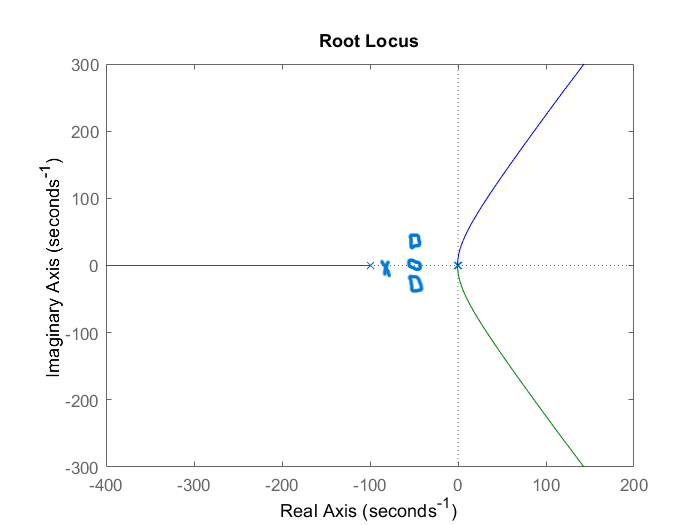
\includegraphics[scale=0.7]{Resources/5.png}
    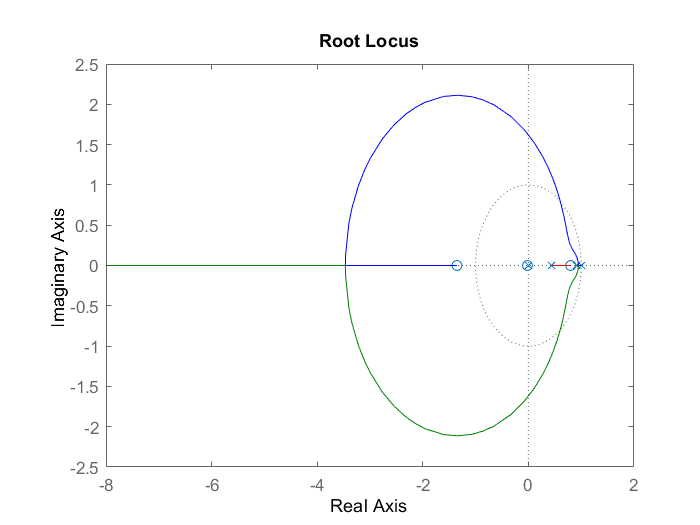
\includegraphics[scale=0.7]{Resources/6.png}
    
    \begin{problem}{سوال پنجم}
    	\raggedleft
    	$D(1) = 1 + 0.05K - 1.2 + 0.07K + 0.2 + 0.005K^2 - 0.007K $
    	
    	$0.005K^2 + 0.127K > 0$
    	
    	$K(0.005K + 0.127) > 0$
    	
    	$K < -25.4 , K > 0$
    	
    	$D(-1) = -1 + 0.05K - 1.2 - 0.07 - 0.2 + 0.005K^2 - 0.007K$
    	
    	$0.005K^2 $
    
    \end{problem}
    
    \begin{problem}{سوال ششم}
    	\raggedleft
    	\lr{First Evaluate the sufficient conditions:}
    	
    	\begin{align}
    		& \sum\limits_{i=1}^{3}{\frac{{{C}_{i}}}{{{T}_{i}}}\le n({{2}^{\frac{1}{n}}}-1)} \nonumber \\ 
    		& \to (\frac{1}{3}+\frac{2}{8}+\frac{5}{20})\le 3({{2}^{\frac{1}{3}}}-1) \nonumber \\ 
    		& 0.83\le 0.7797 \nonumber 
    	\end{align}
    	
    	\lr{It is clearly not satisfied.}
    	
    	\lr{Let's analyze other sufficient conditions:}
    	
    	\begin{align}
    		& \prod\limits_{i=1}^{3}{(\frac{{{C}_{i}}}{{{T}_{i}}}+1)\le 2} \nonumber \\ 
    		& \to (\frac{1}{3}+1)(\frac{2}{8}+1)(\frac{5}{20}+1)\le 2 \nonumber \\ 
    		& 2.08\le 2 \nonumber 
    	\end{align}
    	
    	\lr{It is not satisfied either, so let's move to the necessary conditions.}
    	
    	$R_i \le D_i$
    	
    	\centering
    	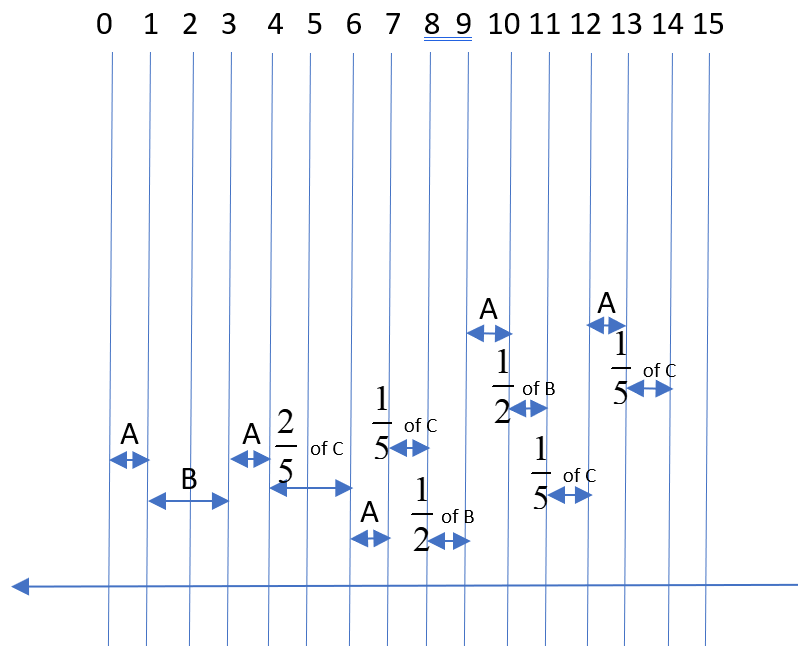
\includegraphics[scale=0.8]{Resources/4.png}
    	
    	\raggedleft
    	\lr{Hence, the tasks are schedulable with the RM algorithm }
    	
    	
    	
    	
    	
    \end{problem}


\end{document}
